\chapter{Результаты решения задачи 3D локализации}

\section{Используемые данные}

В качестве датасета использовался не LIDC-IDRI непосредственно, как это было сделано в решении задачи 2d-сегментации, а его подможество LUNA \cite{luna}, содержащее 888 сканов в формате MetalImage и 1187 опухолей, каждая из которых представленна в виде bounding box. В отличие от LIDC-IDRI из LUNA исключены сканы, по толщине превосходящие 2.5 мм, а также включены только те опухоли, которые были размечены хотя бы тремя и четырех специалистов-радиологов. Еще одна особенность LUNA по сравнению с LIDC состоит в том, что средний размер новообразований в LUNA составляет 8.3 мм при стандартном отклонении в 4.8 мм, когда для LIDC-IDRI эти показатели составляют 12.8мм и 10.6 мм соответствено.

\section{Детали реализации}

\subsection{Реализация DeepSEED}

В оригинальной работе было предложено подавать на вход сети обрезанные участки КТ изображений размера $128^3$, однако такая размерность входных данный требует вычислительных ресурсов, которые были недоступны во время реализации, что привело к уменьшению размерности входа до $64^3$.


\subsection{Реализация Адаптивной нормализации}

Адаптивная нормализация была добавлена в сеть вместо батчевой нормализации. Она применяется после всех блоков (свертка, активация) и в кодировщике, и в декодировщике кроме первого слоя. В качестве входа $x$ формулы \eqref{eq:adain} используется тензор, полученный на выходе активации, а в качестве параметра $y$ используется выход побочной сети, имеющей простую архитектуру - 3 полносвязных слоя, причем первые два разделены между всеми побочными сетями. Данная архитектура позволяет выявить эффективные параметры афинного преобразования посредством обучения.

\subsection{Реализация CGAN}

Изначально архитектура CGAN, формат и размерность входных и выходных данных были полностью заимствованы у авторов \cite{mirsky} в качестве бейслайн решения. Отметим, что при обучении генератора авторы использовали не стандартную функцию потерь, а комбинированную:

\begin{equation}
L(o, g, D_{output}, labels) = MSE(o, g) + MAE(o, g) + L_{G}(D_{output}, labels)
\end{equation}

$o, g$ - оригинальное и генерированное изображения, соответствующие одному контексту.

$L_{GAN}$ - это стандартная функция потерь генератора, рассчитываемая на выходах дискриминатора и реальных метках объектов. Посредством уменьшения данной функции потерь генератор непосредственно стремится обмануть диксриминатор. Однако наряду с этим авторы предлагают использовать функцию потерь, минимизирующую различия между оригинальными изображениями и генерированными.

Я обучил несколько моделей с полностью заимствованными параметрами, но во время обучения и оценки результатов было обнаружено несоклько проблем:

\begin{enumerate}
    \item Функция потерь дискриминатора оптимизировалась гораздо лучше, чем функция потерь генератора, и начиная с некоторой эпохи, дискриминатор почти всегда отличал генерированные изображения от оригинальных.
    
    \item Выходные изображения были достаточно четкими в области контекста, однако в области латентного входа, где предполагалось генерировать непосредственно опухоль, изображения были мутные.
    
    \item Некоторые модели генерировали очень похожие результаты на различных входах. Данная проблема известна как mode collapse.
\end{enumerate}

Для борьбы с данными проблемами было предпринято несколько различных модификаций сети

\begin{enumerate}
    \item Вариация соотношения числа обновлений генератора и дискриминатора
    \item Увеличение размерности входа 
    \item Вариация функции потерь
\end{enumerate}

\subsubsection{Вариация соотношения числа обновлений генератора и дискриминатора}

Данный подход является стандартным для решения ситуации, когда либо генератор, либо дискриминатор отстает от другого и обучается существенно медленнее, либо совсем не обучается, и функция потерь даже возрастает. В моделях бейслайн архитектуры функции потерь и генератора и дискриминатора уменьшались, однако точность дискриминатора достигала 100\% и далее не уменьшалась. Несмотря на то, что генератору не удавалось обмануть дискриминатор, обучениие продолжало происходить в связи с присутствием $MSE$ и $MAE$ компонент. Данный подход кажется неудовлетворительным, поскольку в таком случае роль дискриминатора фактически отпадает и генератор просто стремится произвести похожее на оригинал изображение.

При увеличении соотношения числа обновлений с $1:1$ до $10:1$ в пользу генератора удалось получить визуально лучшие результаты


\section{Результаты}

\subsection{Результаты локализации с помощью DeepSEED}

В качестве метрик качества были выбраны ROC и FROC кривые. Стоит отметить, что FROC-анализ является достаточно популярным в области локализации новообразований легких. FROC-кривая аналогична ROC-кривой, но по оси $x$ отмечен не процент ложно положительных результатов, а среднее количество ложно-положительных bounding-box-ов на один скан.

Для визуализации результатов на рисунках \ref{roc-baseline} и \ref{froc-baseline} предоставлены графики, полученные в результате тестирования обученной модели.

\begin{figure}[!h]
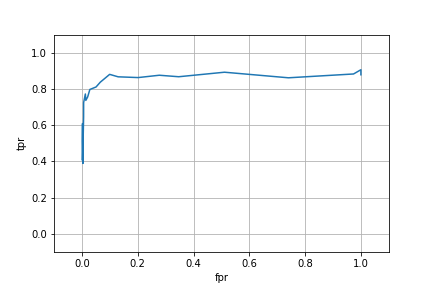
\includegraphics[width=\linewidth]{images/roc.png}
\caption{ROC результаты}\label{roc-baseline}
\centering
\end{figure}

\begin{figure}[!h]
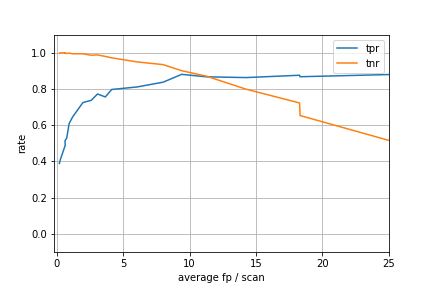
\includegraphics[width=\linewidth]{images/froc.png}
\caption{FROC результаты}\label{froc-baseline}
\centering
\end{figure}

Интересно также сравнить FROC кривые полученные нами и авторами оригинальной статьи. На рисунке \ref{froc-lifan} приведена FROC-кривая из оригинальной статьи.

\begin{figure}[!h]
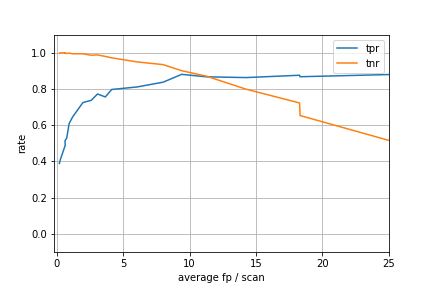
\includegraphics[width=\linewidth]{images/froc.png}
\caption{FROC-результаты (Li, Fan)}\label{froc-lifan}
\centering
\end{figure}

Стоит отметить схожесть кривых. Полученные результаты оказались несколько хуже результатов в статье, что возможно объяснить вынужденным сокращением размерностей обрезанных изображений, подаваемых на вход DeepSEED.

\subsection{Результаты обучения CGAN}

Для оценки качеcтва работы сети CGAN в первую очередь применялся визуальный анализ. На рисунке \ref{mirskiy-results} представлены примеры генерированных изображений, заимствованные из работы Мирского и др. На рисунке \ref{cgan-baseline-results} представлены результаты работы CGAN, предложенной в статье, но обученной нами. На рисунке \ref{cgan-adain-results} представлены результаты работы CGAN, в архитектуру которого вместо BN добавлен AdaIN

\begin{figure}[!h]
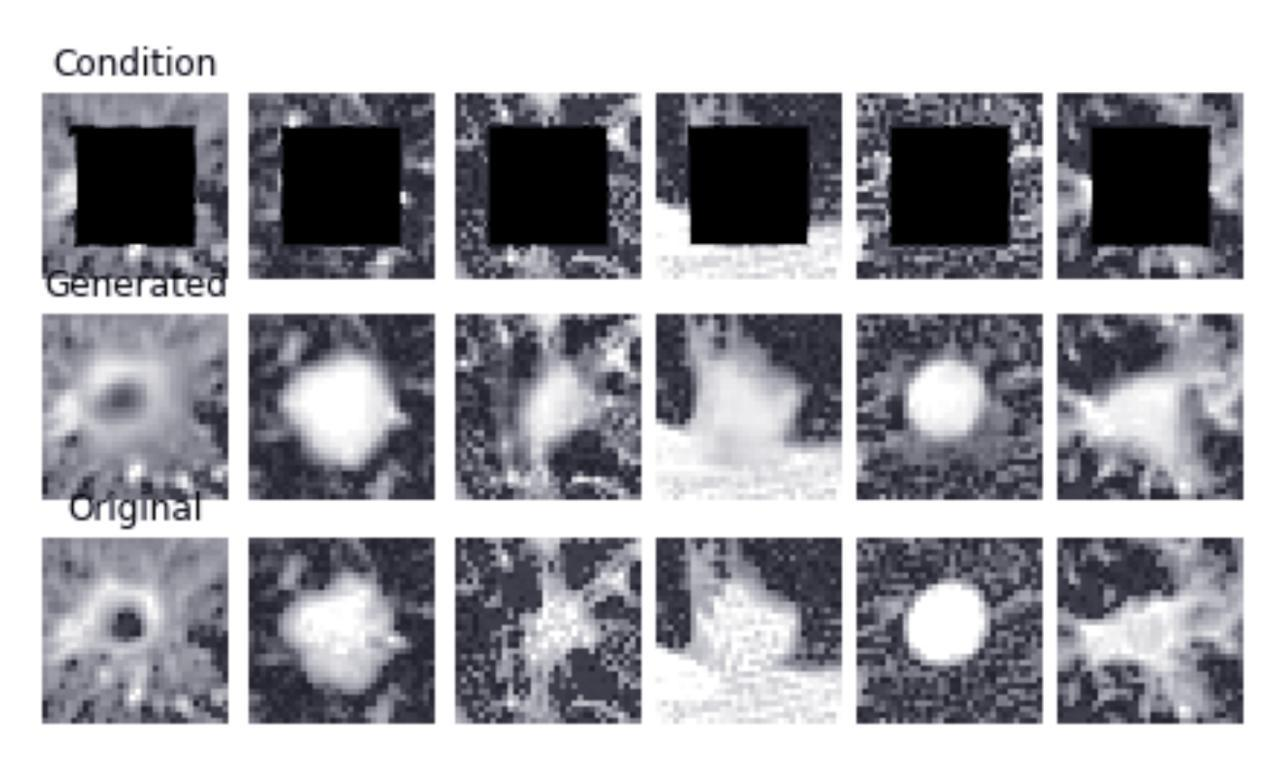
\includegraphics[width=\linewidth]{images/mirskiy-results.jpg}
\caption{Пример генерированных изображений (Mirsky et.al.)}\label{mirskiy-results}
\centering
\end{figure}

\begin{figure}[!h]
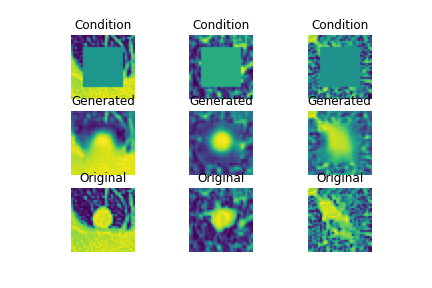
\includegraphics[width=\linewidth]{images/no-adain.png}
\caption{Пример генерированных изображений (Без AdaIN)}\label{cgan-baseline-results}
\centering
\end{figure}

\begin{figure}[!h]
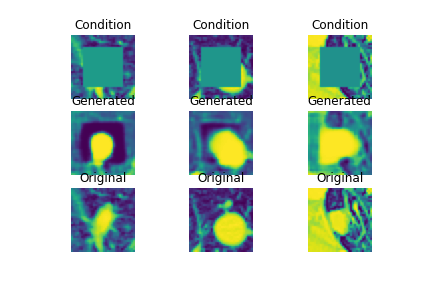
\includegraphics[width=\linewidth]{images/adain.png}
\caption{Пример генерированных изображений (С использованием AdaIN)}\label{cgan-adain-results}
\centering
\end{figure}